\section{Methodology}

The workflow of our project can be divided into five different stages:
Exploratory Data Analysis (EDA), Data Partitioning, Dimensionality Reduction,
Models, and Metrics. Figure \ref{fig:fig1}, displays a generalized view on
these stages.

\begin{figure}[H]
	\begin{center}
		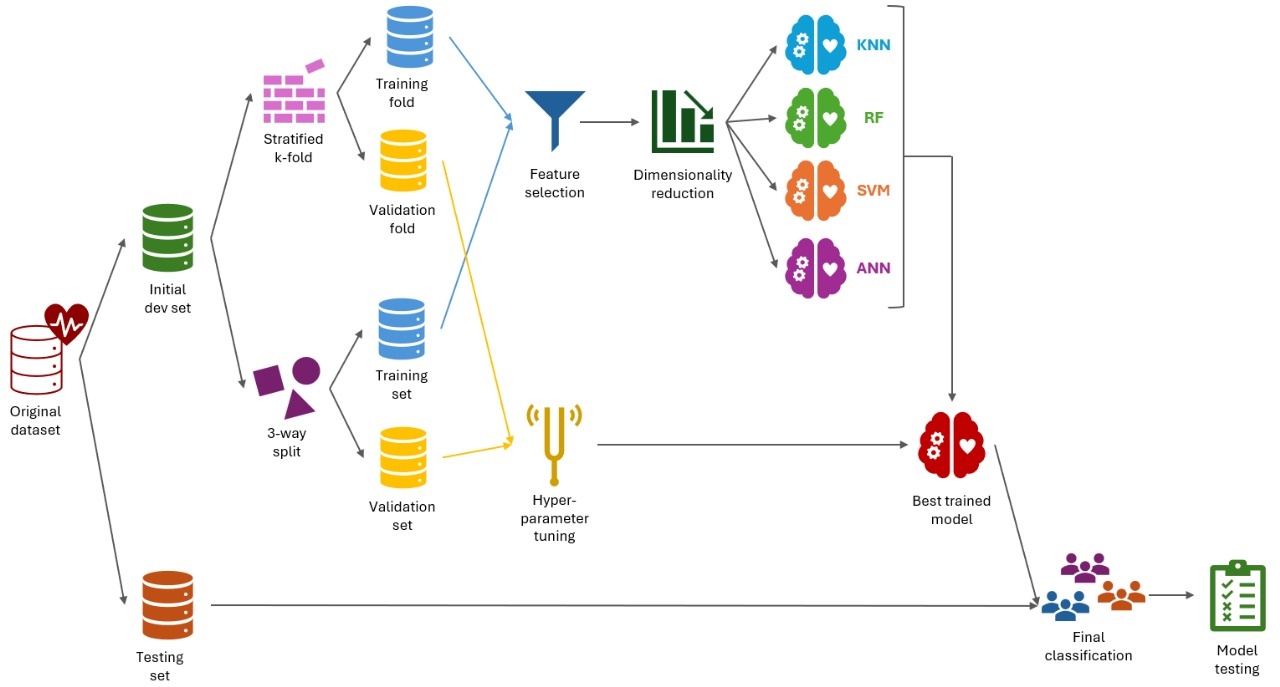
\includegraphics[width=0.99\textwidth, height=7.2cm]{../images/schemas/workflow_01.jpeg}
	\end{center}
	\caption{Methodology schema.}
	\label{fig:fig1}
\end{figure}

\subsection{Exploratory Data Analysis (EDA)}

\subsubsection{Dataset Description}

The ACDC dataset is well-curated, with no missing values and 20 patients per
class across five categories: Dilated Cardiomyopathy (DCM), Hypertrophic
Cardiomyopathy (HCM), Myocardial Infarction (MINF), Normal (NOR), and Right
Ventricular abnormality (RV). Only weight and height were provided for
demographics, so we computed the Body Mass Index (BMI) to analyze their
distribution across classes, defined as:

\begin{align}
	\text{BMI} = \frac{\text{Weight (kg)}}{\text{Height (m)}^2}.
\end{align}

The BMI distributions across classes are shown in Figure \ref{fig:figA1}. We
observe that most patients across all classes fall within the normal and
overweight BMI ranges. HCM patients tend to have higher BMI values, with
several falling into the obese categories, while RV patients generally show
lower BMI values compared to other groups.

\subsubsection{Outliers Detection}

Next, we checked for the presence of outliers using the Interquartile Range
(IQR) method. A value $x$ is defined as an outlier if it satisfies the
condition:

\begin{align}
	x < Q_1 - 1.5 \times \text{IQR} \quad \text{or} \quad x > Q_3 + 1.5 \times \text{IQR},
\end{align}

where the IQR is given by $Q_3 - Q_1$. In Figure \ref{fig:figA2}, we show the
number of outliers detected per class for the top ten features with the highest
total outlier counts. Given that each class has 20 observations per feature, an
average of approximately one outlier per class suggests that outliers are
sparse and evenly distributed. Therefore, we conclude that no outlier removal
is necessary.

\subsubsection{Normalization}

For normalization, we applied the \texttt{StandardScaler} method. Prior to
this, we used the Shapiro-Wilk test to verify that the features approximately
followed a Gaussian distribution. Figure \ref{fig:figA3} presents Q-Q plots and
corresponding \( p \)-values, showing that most features reasonably follow a
normal distribution. \texttt{StandardScaler} transforms each feature \( x \)
according to:

\begin{align}
	z = \frac{x - \mu}{\sigma},
\end{align}

where \( \mu \) is the mean and \( \sigma \) is the standard deviation of the
feature. This ensures that each feature has a mean of zero and a standard
deviation of one.

\subsubsection{Correlation Analysis}

Finally, we computed the Pearson correlation coefficient between each radiomic
feature and the class labels. Since the target variable is categorical with
five classes, we applied a One-vs-Rest (OvR) strategy, where each class was
binarized and analyzed independently against the rest. For a given class, the
correlation was computed as:

\begin{align}
	r = \frac{\sum (x_i - \bar{x})(y_i - \bar{y})}{\sqrt{\sum (x_i - \bar{x})^2} \sqrt{\sum (y_i - \bar{y})^2}},
\end{align}

where \( x \) represents the feature values and \( y \) the binary labels (one
for the class of interest, zero otherwise). Figure \ref{fig:figA4} shows the
top five most correlated features for each class. Shape and texture descriptors
are the most prominent among the highly correlated features. However, what is
evident is the high level of multicollinearity among the radiomic features, as
shown in Figure \ref{fig:figA5}.

\subsection{Data Partitioning}

\subsubsection{Simple Split}

In the Simple Split strategy, the dataset was initially divided into 80\% for
training and validation, and 20\% for testing. The 80\% training-validation
portion was further split into 75\% for training and 25\% for validation,
resulting in final proportions of 60\% training, 20\% validation, and 20\%
testing (Figure \ref{fig:figA6}). This 80/20 split is a widely accepted
convention in machine learning, particularly for small to medium-sized
datasets, as it provides a practical balance between allocating sufficient data
for model training and retaining enough data to evaluate performance on
previously unseen cases \cite{beyond8020}.

\subsubsection{Stratified K-Fold}

For the Stratified K-Fold strategy, we again used the initial 80\% of the data
for training and validation, resulting in 80 samples, corresponding to 16
samples per class (\( 80/5 = 16 \)). We then applied cross-validation while
maintaining class balance. Although \( k=5 \) is often considered a gold
standard for small medical imaging datasets to balance bias and variance
\cite{vabalas2019}, we selected \( k=4 \) to better match the dataset
structure. This ensured that each class contributed 12 samples for training and
4 samples for validation across the folds, as shown in Figure \ref{fig:figA7}.

\subsection{Dimensionality Reduction}

\subsubsection{Modified Least Absolute Shrinkage and Selection Operator (LASSOmodf)}

To address the strong multicollinearity and redundancy typical of radiomic
features, we adopted a multi-stage feature selection strategy \cite{wang2023}.
First, variance filtering was applied to remove features with zero variance.
Then, an ANOVA F-test was performed to retain features with statistically
significant differences across classes, selecting those with \( p < 0.05 \).
Subsequently, a sparse model was obtained by solving the LASSO optimization
problem:

\begin{align}
	J(\mathbf{h}) = \sum_{i=1}^{m} \left( y^{(i)} - \sum_{j=0}^{n} h_j x^{(i)}_j \right)^2 + \lambda \sum_{j=0}^{n} \lvert h_j \rvert,
\end{align}

where \( x^{(i)} \) and \( y^{(i)} \) represent the features and label of the
\(i\)-th sample, \( \mathbf{h} \) are the regression coefficients, and \(
\lambda \) controls sparsity. The LASSO coefficient trajectories across
different values of \(\lambda\) are illustrated in Figure \ref{fig:figA8}.

Both the regularization parameter \(\lambda\) and the coefficient threshold
\(\text{coe\_thr}\) were optimized through a similar grid search procedure: for
each candidate value, the Mean Squared Error (MSE) on a validation subset was
computed and the value minimizing MSE was selected, as shown in Figures
\ref{fig:figA9} and \ref{fig:figA10}. Specifically, the validation MSE for a
given parameter \(\theta\) was computed as:

\begin{align}
	\text{MSE}(\theta) = \frac{1}{|D_{\text{val}}|} \sum_{i \in D_{\text{val}}}\left( y^{(i)} - \hat{y}^{(i)}(\theta) \right)^2,
\end{align}

where \(D_{\text{val}}\) is the validation subset, \(\theta\) corresponds
either to \(\lambda\) or to \(\text{coe\_thr}\), and \(\hat{y}^{(i)}(\theta)\)
denotes the prediction under the given parameter. For coefficient thresholding,
after fitting the LASSO model with the optimal \(\lambda_{\text{opt}}\), the
threshold \(\text{coe\_thr}\) was varied between the minimum and maximum
absolute coefficients:

\begin{align}
	h_{\text{max}} & = \max_{j} \lvert h_j \rvert, \quad
	h_{\text{min}} = \min_{j} \lvert h_j \rvert
\end{align}

retaining features satisfying \(\lvert h_j \rvert >
\text{coe\_thr}_{\text{opt}}\) for the final feature subset.

\subsubsection{Linear Discriminant Analysis (LDA)}

Following feature selection, the retained features were further reduced in
dimensionality using Linear Discriminant Analysis (LDA). LDA is a supervised
technique that projects the data onto a lower-dimensional space by maximizing
the separation between classes while minimizing the variance within each class.
Since our dataset contains five classes, LDA can reduce the feature space to at
most \(5 - 1 = 4\) dimensions. Alternative methods like Principal Component
Analysis (PCA) were not considered optimal, as our goal was not to interpret
individual features but to maximize class separability. Additionally,
collinearity had already been addressed during feature selection, making PCA's
variance-based transformation unnecessary.

\subsection{Models}

\subsubsection{k-Nearest Neighbors (KNN)}

The first supervised model applied was the k-Nearest Neighbors (KNN)
classifier. KNN predicts the class of a new sample based on the majority class
among its \(k\) closest neighbors in the feature space. It is a non-parametric,
instance-based learning algorithm that relies on distance comparisons rather
than a formal training phase. While not expected to be the most accurate model,
its simplicity makes it a useful baseline for comparison. In
\cite{pandey2023knn}, KNN was selected for its interpretability and
effectiveness on small radiomic datasets, particularly when feature space was
already reduced like our case.

\subsubsection{Random Forest (RF)}

The second supervised model applied was the Random Forest (RF) classifier. RF
is an ensemble learning method that constructs multiple decision trees using
random subsets of the data and features, combining their predictions through
majority voting. It is well-suited for modeling non-linear interactions and is
robust to feature correlations, making it effective in handling complex
relationships within radiomic data. Li et al. \cite{li2020rf} demonstrated
similar benefits when applying RF to predict treatment outcomes from radiomic
features in cervical cancer, citing the model’s stability and good
generalization on structured imaging data.

\subsubsection{Support Vector Machine (SVM)}

The third supervised model applied was the Support Vector Machine (SVM)
classifier. SVM is a supervised learning algorithm that aims to find the
optimal hyperplane that separates classes by maximizing the margin between the
closest data points of different classes, known as support vectors. In our
pipeline, SVM was a suitable choice because the dimensionality reduction
ensured a compact feature space, allowing SVM to effectively maximize class
separation. This is supported by the findings of Xu et al. \cite{xu2019svm},
who employed SVM for lymph node metastasis prediction using radiomics.

\subsubsection{Artificial Neural Network (ANN)}

The last supervised model applied was the Artificial Neural Network (ANN). ANNs
consist of interconnected layers of neurons, where each neuron computes a
weighted sum of its inputs followed by a non-linear activation function.
However, typically they require careful tuning and regularization to prevent
overfitting, especially when working with limited data. In a related study,
Mulet de los Reyes et al. \cite{mulet2023ann} demonstrated the ability of ANNs
to perform robust tumor segmentation from radiomic inputs by leveraging feature
learning. Their findings suggest that when paired with appropriate
preprocessing and dimensionality reduction, ANNs can effectively learn from
structured imaging-derived datasets.

\subsection{Metrics}

\subsubsection{Model Selection}

During hyperparameter tuning, models were evaluated using a custom score
designed to balance generalization and overfitting:

\begin{align}
	\text{Score} = \text{Validation Acc.} - p \times \lvert \text{Training Acc.} - \text{Validation Acc.} \rvert,
\end{align}

where \( p = 0.5 \) controls the penalty for overfitting. The best
hyperparameters were selected by maximizing this score, encouraging models with
high validation performance and low overfitting.

\subsubsection{Model Evaluation}

After training, the following evaluation metrics were computed to evaluate the
model's performance on the test set (Table \ref{tab:tab1}):

\begin{table}[H]
	\centering
	\caption{Evaluation metrics used for model assessment.}
	\label{tab:tab1}
	\begin{adjustbox}{max width=0.99\textwidth}
		\begin{tabular}{p{2.5cm} p{8cm} >{\centering\arraybackslash}p{6cm}}
			\toprule
			\centering\textbf{Metric}    & \textbf{Definition}                                                                                   & \textbf{Formula} \\
			\midrule
			\centering Accuracy (Macro)  & Measures the overall proportion of correctly classified samples, averaged equally across all classes. &
			\(\displaystyle \frac{1}{C} \sum_{c=1}^{C} \frac{\text{TP}_c + \text{TN}_c}{\text{TP}_c + \text{FP}_c + \text{FN}_c + \text{TN}_c}\)                    \\

			\centering Precision (Macro) & Measures the ability of the model to correctly identify positive instances across all classes.        &
			\(\displaystyle \frac{1}{C} \sum_{c=1}^{C} \frac{\text{TP}_c}{\text{TP}_c + \text{FP}_c}\)                                                              \\

			\centering Recall (Macro)    & Measures the ability of the model to capture all relevant instances for each class.                   &
			\(\displaystyle \frac{1}{C} \sum_{c=1}^{C} \frac{\text{TP}_c}{\text{TP}_c + \text{FN}_c}\)                                                              \\

			\centering F1-Score (Macro)  & Harmonic mean between precision and recall, providing a balance between the two.                      &
			\(\displaystyle \frac{1}{C} \sum_{c=1}^{C} 2 \times \frac{\text{Precision}_c \times \text{Recall}_c}{\text{Precision}_c + \text{Recall}_c}\)            \\
			\bottomrule
		\end{tabular}
	\end{adjustbox}
\end{table}

In addition to the overall metrics, the confusion matrix, Receiver Operating
Characteristic (ROC-AUC) curves, and class-wise performance metrics were also
evaluated.
